\documentclass[12pt,a4paper]{article}
\usepackage[a4paper,top=15mm,bottom=15mm,left=16mm,right=16mm]{geometry}
\usepackage[T1]{fontenc}
\usepackage{amsmath}
\usepackage{amssymb}
\usepackage{array}
\usepackage{tikz}
\usetikzlibrary{arrows.meta}

\pagestyle{empty}
\setlength{\parindent}{0pt}
\setlength{\parskip}{4pt}
\allowdisplaybreaks

% A topic from the revision list, with its "Remember" line from the
% revision guide.
\newcommand{\ptitle}[2]{%
  \par\addvspace{10pt}
  \noindent\rule{\linewidth}{0.8pt}\par\nobreak\vspace{1pt}
  \noindent{\large\bfseries #1}\par\nobreak\vspace{1pt}
  \noindent\textbf{Remember: #2}\par\nobreak\vspace{1pt}
  \noindent\rule{\linewidth}{0.4pt}\par\nobreak\vspace{4pt}}
\newcommand{\wq}[1]{\par\addvspace{6pt}\noindent\textbf{Q#1.}\ }

% An operation written under both sides, between the lines of working.
\newcommand{\op}[1]{{\scriptstyle #1}}

% \numline{<from>}{<to>}{<drawing>}: a number line, with the drawing
% placed at height 4, above the line.
\newcommand{\numline}[3]{%
  \begin{tikzpicture}[x=7mm,y=1mm]
    \draw[{Stealth[length=1.5mm]}-{Stealth[length=1.5mm]}] (#1-0.6,0) -- (#2+0.6,0);
    \foreach \n in {#1,...,#2}{\draw (\n,-1) -- (\n,1); \node[below,font=\small] at (\n,-1) {$\n$};}
    #3
  \end{tikzpicture}}
\newcommand{\opencircle}[1]{\draw[thick,fill=white] (#1,4) circle (1.2mm);}
\newcommand{\filledcircle}[1]{\fill (#1,4) circle (1.2mm);}

\begin{document}

\begin{center}
{\Large\bfseries Inequalities}\\[3pt]
{\large Revision questions: worked solutions}
\end{center}

% ----------------------------------------------------------------
\ptitle{Reading and drawing inequalities on number lines}{Open circle: not included.\ \ Filled circle: included.}

\wq{1} (a) Open circle at 1, arrow to the right: $x>1$

(b) Filled circle at $-2$, arrow to the left: $x\le-2$

(c) Filled circle at $-3$ and open circle at 2: $-3\le x<2$

\wq{2} (a) $\ge$ includes 4, so a filled circle at 4, with an arrow to the right.

\numline{-1}{8}{\draw[very thick,-{Stealth[length=1.8mm]}] (4,4) -- (8.6,4); \filledcircle{4}}

(b) $-1$ is not included (open circle), and 5 is included (filled circle).

\numline{-3}{7}{\draw[very thick] (-1,4) -- (5,4); \opencircle{-1} \filledcircle{5}}

\wq{3} (a) $-1$ is not included, and 5 is included: 0, 1, 2, 3, 4, 5

(b) Neither end is included: $-4$, $-3$, $-2$

\wq{4} ``At least 1'' includes 1, and ``less than 5'' does not include 5: $1\le t<5$

\numline{-1}{7}{\draw[very thick] (1,4) -- (5,4); \filledcircle{1} \opencircle{5}}

% ----------------------------------------------------------------
\ptitle{Solving inequalities}{Solve it like an equation, but keep the sign.}

\wq{5}
\[
\begin{array}{r@{\;}c@{\;}l}
  x+7 & > & 12\\
  \op{-7} & & \op{-7}\\
  x & > & 5
\end{array}
\qquad
\begin{array}{r@{\;}c@{\;}l}
  4x & \le & 28\\
  \op{\div4} & & \op{\div4}\\
  x & \le & 7
\end{array}
\qquad
\begin{array}{r@{\;}c@{\;}l}
  2x-3 & < & 11\\
  \op{+3} & & \op{+3}\\
  2x & < & 14\\
  \op{\div2} & & \op{\div2}\\
  x & < & 7
\end{array}
\qquad
\begin{array}{r@{\;}c@{\;}l}
  \frac{x}5+2 & \ge & 4\\
  \op{-2} & & \op{-2}\\
  \frac{x}5 & \ge & 2\\
  \op{\times5} & & \op{\times5}\\
  x & \ge & 10
\end{array}
\]

\wq{6} Expand the bracket first: $3x-6>12$.
\[
\begin{array}{r@{\;}c@{\;}l}
  3x-6 & > & 12\\
  \op{+6} & & \op{+6}\\
  3x & > & 18\\
  \op{\div3} & & \op{\div3}\\
  x & > & 6
\end{array}
\]
\numline{2}{10}{\draw[very thick,-{Stealth[length=1.8mm]}] (6,4) -- (10.6,4); \opencircle{6}}

% ----------------------------------------------------------------
\ptitle{Solving inequalities with the unknown on both sides}{Take away the smaller $x$-term from both sides first.}

\wq{7}
\[
\begin{array}{r@{\;}c@{\;}l}
  5x+2 & > & 3x+10\\
  \op{-3x} & & \op{-3x}\\
  2x+2 & > & 10\\
  \op{-2} & & \op{-2}\\
  2x & > & 8\\
  \op{\div2} & & \op{\div2}\\
  x & > & 4
\end{array}
\qquad
\begin{array}{r@{\;}c@{\;}l}
  8x-1 & \le & 5x+11\\
  \op{-5x} & & \op{-5x}\\
  3x-1 & \le & 11\\
  \op{+1} & & \op{+1}\\
  3x & \le & 12\\
  \op{\div3} & & \op{\div3}\\
  x & \le & 4
\end{array}
\qquad
\begin{array}{r@{\;}c@{\;}l}
  2x+8 & < & x+13\\
  \op{-x} & & \op{-x}\\
  x+8 & < & 13\\
  \op{-8} & & \op{-8}\\
  x & < & 5
\end{array}
\]
In (c) we expand the bracket first: $2(x+4)=2x+8$.

% ----------------------------------------------------------------
\ptitle{Solving double inequalities}{Whatever you do to one part, do to all three parts.}

\wq{8}
\[
\begin{array}{r@{\;}c@{\;}c@{\;}c@{\;}l}
  5 & < & x+3 & \le & 9\\
  \op{-3} & & \op{-3} & & \op{-3}\\
  2 & < & x & \le & 6
\end{array}
\qquad
\begin{array}{r@{\;}c@{\;}c@{\;}c@{\;}l}
  -6 & \le & 3x & < & 9\\
  \op{\div3} & & \op{\div3} & & \op{\div3}\\
  -2 & \le & x & < & 3
\end{array}
\qquad
\begin{array}{r@{\;}c@{\;}c@{\;}c@{\;}l}
  1 & < & 2x-5 & < & 9\\
  \op{+5} & & \op{+5} & & \op{+5}\\
  6 & < & 2x & < & 14\\
  \op{\div2} & & \op{\div2} & & \op{\div2}\\
  3 & < & x & < & 7
\end{array}
\]
(a) 3, 4, 5, 6\qquad (b) $-2$, $-1$, 0, 1, 2\qquad (c) 4, 5, 6

\wq{9}
\[
\begin{array}{r@{\;}c@{\;}c@{\;}c@{\;}l}
  -7 & < & 4n+1 & \le & 13\\
  \op{-1} & & \op{-1} & & \op{-1}\\
  -8 & < & 4n & \le & 12\\
  \op{\div4} & & \op{\div4} & & \op{\div4}\\
  -2 & < & n & \le & 3
\end{array}
\]
$-2$ is not included, so the smallest integer is $-1$. 3 is included, so the largest is 3.

% ----------------------------------------------------------------
\ptitle{Constructing inequalities}{At most $\le$,\ \ at least $\ge$,\ \ more than $>$,\ \ less than $<$.}

\wq{10} ``More than'' is $>$.
\[
\begin{array}{r@{\;}c@{\;}l}
  3n-4 & > & 20\\
  \op{+4} & & \op{+4}\\
  3n & > & 24\\
  \op{\div3} & & \op{\div3}\\
  n & > & 8
\end{array}
\]

\wq{11} The cost is $3+2m$, and Ella can spend at most £19, so $\le$.
\[
\begin{array}{r@{\;}c@{\;}l}
  3+2m & \le & 19\\
  \op{-3} & & \op{-3}\\
  2m & \le & 16\\
  \op{\div2} & & \op{\div2}\\
  m & \le & 8
\end{array}
\]
The greatest whole number of miles is 8.

\wq{12} Perimeter $=x+(x+6)+x+(x+6)=4x+12$. ``At least'' is $\ge$.
\[
\begin{array}{r@{\;}c@{\;}l}
  4x+12 & \ge & 40\\
  \op{-12} & & \op{-12}\\
  4x & \ge & 28\\
  \op{\div4} & & \op{\div4}\\
  x & \ge & 7
\end{array}
\]
The smallest possible value of $x$ is 7.

% ----------------------------------------------------------------
\ptitle{Inequalities on graphs}{Dashed: not on it.\ \ Solid: on it.\ \ Test a point.}

\wq{13} (a) The line is $x=3$, solid, and the region is to the left: $x\le3$

(b) The line is $y=-1$, dashed, and the region is above: $y>-1$

(c) The line is $y=x+1$, solid, and the region is above. Test $(0,3)$: $3\ge0+1$ \checkmark, so $y\ge x+1$

\wq{14} $y=1$ is solid and R is above it: $y\ge1$.\quad $x=4$ is dashed and R is to its left: $x<4$.\quad $y=x$ is solid and R is below it: $y\le x$.

Test a point in R, $(3,2)$: $2\ge1$ \checkmark,\ \ $3<4$ \checkmark,\ \ $2\le3$ \checkmark

\wq{15} The three lines are $x=0$ (the $y$-axis), $y=1$ and $x+y=4$, all solid. The region is the triangle with corners $(0,1)$, $(3,1)$ and $(0,4)$.

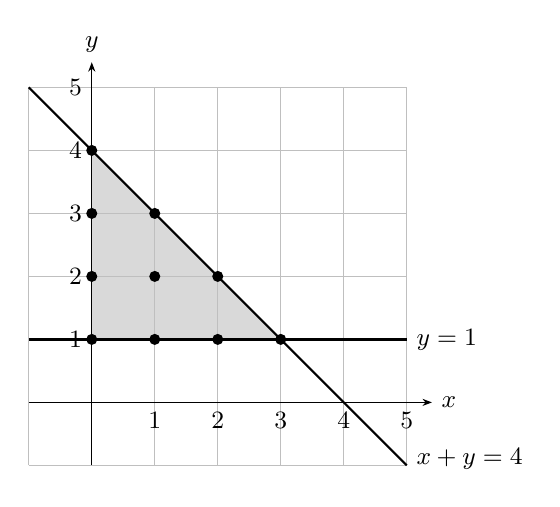
\begin{tikzpicture}[x=8mm,y=8mm,font=\small]
  \fill[black!15] (0,1) -- (3,1) -- (0,4) -- cycle;
  \draw[black!25,step={(1,1)}] (-1,-1) grid (5,5);
  \draw[-{Stealth[length=1.2mm]}] (-1,0) -- (5.4,0) node[right] {$x$};
  \draw[-{Stealth[length=1.2mm]}] (0,-1) -- (0,5.4) node[above] {$y$};
  \foreach \t in {1,...,5}{\node[below] at (\t,0) {\t}; \node[left] at (0,\t) {\t};}
  \draw[thick] (-1,1) -- (5,1);
  \draw[thick] (-1,5) -- (5,-1);
  \node[right] at (5,-0.9) {$x+y=4$};
  \node[right] at (5,1) {$y=1$};
  \foreach \p in {(0,1),(0,2),(0,3),(0,4),(1,1),(1,2),(1,3),(2,1),(2,2),(3,1)}{\fill \p circle (2pt);}
\end{tikzpicture}

Counting the points, including the edges: $4+3+2+1=10$ points.

% ----------------------------------------------------------------
\ptitle{Dividing by a negative number}{Times or divide by a negative? Flip the sign!}

\wq{16}
\[
\begin{array}{r@{\;}c@{\;}l@{\quad}l}
  -2x & > & 8\\
  \op{\div(-2)} & & \op{\div(-2)}\\
  x & < & -4 & \text{\small flipped}
\end{array}
\qquad
\begin{array}{r@{\;}c@{\;}l@{\quad}l}
  -5x & \le & -15\\
  \op{\div(-5)} & & \op{\div(-5)}\\
  x & \ge & 3 & \text{\small flipped}
\end{array}
\qquad
\begin{array}{r@{\;}c@{\;}l@{\quad}l}
  7-3x & < & 1\\
  \op{-7} & & \op{-7}\\
  -3x & < & -6\\
  \op{\div(-3)} & & \op{\div(-3)}\\
  x & > & 2 & \text{\small flipped}
\end{array}
\]

\wq{17} With $x=4$: $10-2\times4=2$, and 2 is not more than 4. So $x=4$ does not work, and Jo's answer $x>3$ is wrong.
\[
\begin{array}{r@{\;}c@{\;}l@{\quad}l}
  10-2x & > & 4\\
  \op{-10} & & \op{-10}\\
  -2x & > & -6\\
  \op{\div(-2)} & & \op{\div(-2)}\\
  x & < & 3 & \text{\small flipped}
\end{array}
\]
Jo divided by $-2$ without flipping the sign.

% ----------------------------------------------------------------
\par\addvspace{10pt}
\noindent\rule{\linewidth}{0.8pt}\par\nobreak\vspace{1pt}
\noindent{\large\bfseries Problem solving}\par\nobreak\vspace{1pt}
\noindent\rule{\linewidth}{0.4pt}\par\nobreak\vspace{4pt}

\wq{18} $3x-1>5$ gives $3x>6$, so $x>2$.\quad $2x+3\le15$ gives $2x\le12$, so $x\le6$.

Both are true when $2<x\le6$: the integers are 3, 4, 5, 6.

\wq{19} The inequality must include $-2$ and 1, but not $-3$ or 2. For example $-3<x<2$, or $-2\le x\le1$.

\wq{20} In pence, plan A costs $1000+5m$ and plan B costs $1800+m$. Plan B is cheaper when
\[
\begin{array}{r@{\;}c@{\;}l}
  1800+m & < & 1000+5m\\
  \op{-m} & & \op{-m}\\
  1800 & < & 1000+4m\\
  \op{-1000} & & \op{-1000}\\
  800 & < & 4m\\
  \op{\div4} & & \op{\div4}\\
  200 & < & m
\end{array}
\]
Plan B is cheaper for more than 200 minutes of calls. (At exactly 200 minutes both plans cost £20.)

\end{document}
